\section{Introduction}
\label{sec:intro}

With the popularity of mobile and potable devices, people are getting easier to sketch objects. Sketches have proved to be a powerful and effective tool for communication. A mount of approaches focused on sketch recognition have been studied. But all of them take the recognition accuracy as their only benchmark with ignorance of recognition speed. Mobile and portable devices have more limited computing resources and storage compared to high-performance server or even personal computer. So it is necessary to promote the speed of sketch recognition, but not only accuracy.

Although sketches and images can be visually recognized, they have two main differences: (i) Patterns take more important place in sketch recognition than in image recognition. Sketches vary largely within class. Meanwhile, some sketches coming from different class have similar looking from the high level. But differences can be told from the mid level or low level, e.g., some cats and snowmen are identified easily from their facial part, but hardly from the whole sketches. Objects in images are from the real life. The size of different parts from one object in images are more rationale than that in sketches. (ii) Sketches are sparser than images. Sketches are generated by a pen. Images are the photos from the life. This means a sketch can be viewed as a series of points.

Previous works on sketch recognition are generally borrowed from image classification paradigm. Both conventional sketch recognition and Deep Neural Networks (DNNs) take sketches as images. These methods do not take full advantage of the sparsity of sketches. Besides, in pursuit of high accuracy, they developed different feature fusion methods without the consideration of the model is too bloated to be distributed in mobile devices. Due to special generalization a sketch, it can be represented by only a series of points which taking less storage than represented as an image.

In this paper, we propose a DNN, SketchPointNet, for accelerating sketch recognition and reducing recognition model size, which derived from PointNet \cite{qi2017pointnet}. However, existing approaches are primarily taking sketches as images and regarding recognition accuracy as their only benchmark. In order to speeding up sketch recognition, we resample each sketch as a series of points. SketchPointNet is designed with two notable characteristic: (i) a group of micro PointNets are encoded in SketchPointNet hierarchically to capture features of different level; and (ii) micro PointNets summarize patterns along the time series points, while image-based DNN's kernels move in two directions.

Our contributions are summarized as follows: (i)for the first time, we take sketches as a series of points and propose a corresponding DNN to recognize them; (ii) we demonstrate that SketchPointNet has a higher recognition speed and a smaller model size than existing DNN-based approaches.

\begin{figure*}
    \center
    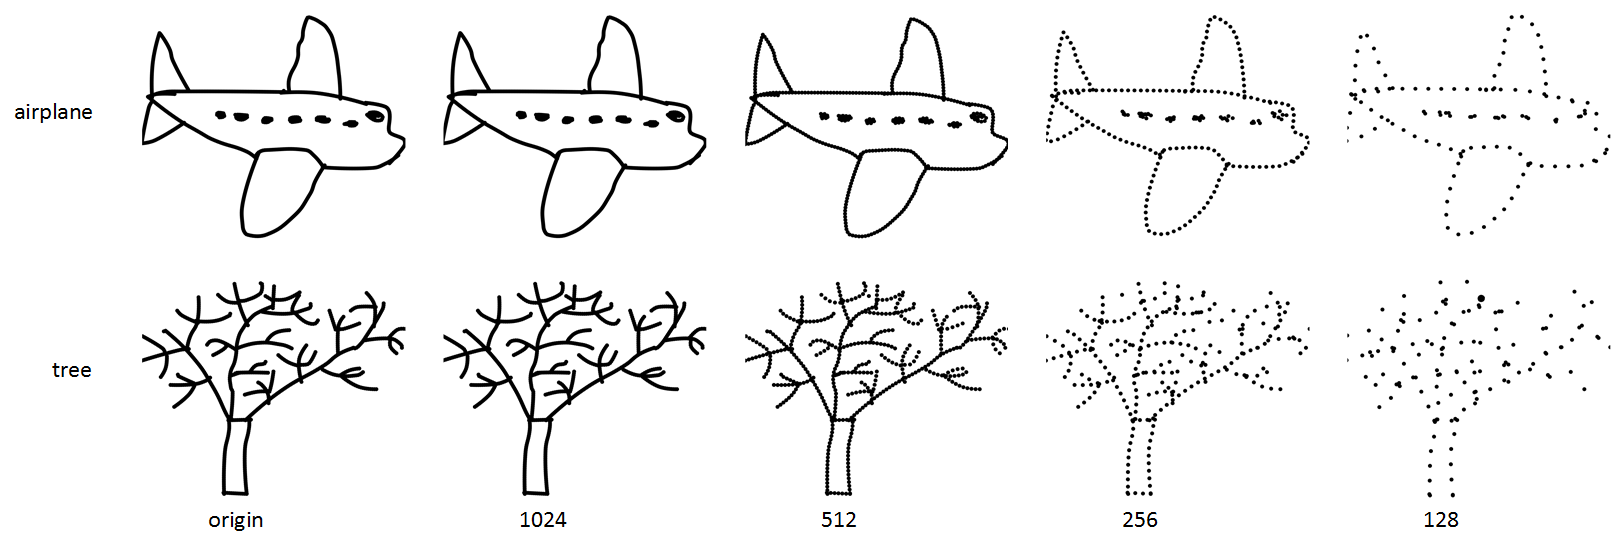
\includegraphics[width=6.5in]{images/resample.png}
    \fcaption{Resample the airplane and the tree into $N$(1024, 512, 256, 128) points.}
    \label{fig:resample}
\end{figure*}
